\chapter{Digital Logic: From Transistors to Adders}\index{digital logic}

Type $6+7$ into your phone's calculator and it answers 13 before your finger leaves the screen. Inside
the phone, there is no one who knows arithmetic. There are only billions of tiny switches, each of
which is either on or off. So how does a pile of switches add?

In this chapter, you will build an adding machine from scratch. You will start with a single
transistor, make a gate called NAND out of four of them, build every other kind of logic from NAND
alone, and finally chain the pieces into a circuit that adds binary numbers. Then you will check your
design in Python.

You already have the pieces. The Sets and Logic chapter gave you logic tables. The Diodes chapter
showed how doping turns silicon into a conductor. The Data Representation chapter showed how numbers
are stored in binary, including negative numbers in two's complement.

\section{Bits as Voltages}\index{bit!as voltage}
A wire in a chip carries a bit as a voltage. A wire near 0 volts means 0 (false). A wire near the
chip's supply voltage, called $V_{dd}$ and often about 1 volt in a modern phone, means 1 (true). In
between is a no-man's-land that a well-designed circuit passes through quickly.

From here on, we write logic tables with 1 and 0 instead of T and F. The tables in this form are
usually called \newterm{truth tables}.\index{truth table}

\section{Transistors Are Switches}\index{transistor}\index{MOSFET}
A \newterm{transistor} is a switch with no moving parts, controlled by a voltage. The kind found in
nearly every chip is the MOSFET. It is a strip of doped silicon with a third terminal, the
\newterm{gate}, sitting just above it behind a thin layer of glass. Putting a voltage on the gate pulls
charge carriers into the silicon under it, opening a path for current. Remove the voltage, and the
path closes.

There are two flavors, and they behave as opposites:
\begin{itemize}
\item An \textbf{nMOS} transistor is \emph{on} (conducting) when its gate is 1.
\item A \textbf{pMOS} transistor is \emph{on} when its gate is 0. Its symbol has a little circle on
the gate, which means ``opposite.''
\end{itemize}

Chips pair the two flavors together, a style called \newterm{CMOS} (complementary MOS). Here is the
simplest CMOS circuit, the \newterm{inverter}:

\begin{figure}[htbp]
\centering
\begin{circuitikz}
\draw (0,0) node[pmos, emptycircle] (p) {};
\draw (0,-2.2) node[nmos] (n) {};
\draw (p.D) -- (n.D);
\draw (p.S) -- ++(0,0.3) node[vcc]{$V_{dd}$};
\draw (n.S) node[ground]{};
\draw (p.G) -- ++(-0.5,0) coordinate (gp);
\draw (n.G) -- ++(-0.5,0) coordinate (gn);
\draw (gp) -- (gn);
\draw ($(gp)!0.5!(gn)$) to[short,*-o] ++(-0.8,0) node[left]{$A$};
\draw ($(p.D)!0.5!(n.D)$) to[short,*-o] ++(1,0) node[right]{out};
\end{circuitikz}
\caption{A CMOS inverter. The pMOS transistor on top connects the output to $V_{dd}$; the nMOS
transistor on the bottom connects it to ground (0 V).}
\label{fig:inverter}
\end{figure}

Trace it. If $A = 1$, the bottom transistor is on and the top one is off, so the output is connected to
ground: out $= 0$. If $A = 0$, the top transistor is on and the bottom is off, so the output is connected
to $V_{dd}$: out $= 1$. The circuit flips its input. It is a NOT gate.

Notice that one transistor is always off, so no current flows straight from $V_{dd}$ to ground. A CMOS
circuit uses power mostly when its outputs switch. This is why your phone can hold billions of
transistors without melting.

\section{The NAND Gate}\index{NAND gate}
Now use four transistors. Put two pMOS transistors side by side (in parallel) between $V_{dd}$ and the
output, and two nMOS transistors one after the other (in series) between the output and ground.

\begin{figure}[htbp]
\centering
\begin{circuitikz}
\draw (0,0) node[pmos, emptycircle] (p1) {};
\draw (2.2,0) node[pmos, emptycircle] (p2) {};
\draw (p1.S) -- ++(0,0.3) coordinate (t1);
\draw (p2.S) -- ++(0,0.3) coordinate (t2);
\draw (t1) -- (t2); \draw ($(t1)!0.5!(t2)$) node[vcc]{$V_{dd}$};
\draw (p1.D) -- ++(0,-0.4) coordinate (m1);
\draw (p2.D) -- ++(0,-0.4) coordinate (m2);
\draw (m1) to[short,*-] (m2);
\draw (0,-2.3) node[nmos] (n1) {};
\draw (0,-4.3) node[nmos] (n2) {};
\draw (m1) -- (n1.D);
\draw (n1.S) -- (n2.D);
\draw (n2.S) node[ground]{};
\draw (m2) to[short,*-o] ++(1,0) node[right]{out};
\draw (p1.G) to[short,-o] ++(-0.4,0) node[left]{$A$};
\draw (n1.G) to[short,-o] ++(-0.4,0) node[left]{$A$};
\draw (p2.G) to[short,-o] ++(-0.4,0) node[left]{$B$};
\draw (n2.G) to[short,-o] ++(-0.4,0) node[left]{$B$};
\end{circuitikz}
\caption{A CMOS NAND gate. Both $A$ wires are the same input, and so are both $B$ wires.}
\label{fig:cmos-nand}
\end{figure}

The output reaches ground only if \emph{both} bottom transistors are on, which needs $A = 1$ and
$B = 1$. In every other case, at least one of the top transistors is on and pulls the output up to 1.

\begin{center}
\begin{tabular}{c c | c}
$A$ & $B$ & $A$ NAND $B$ \\
\hline
0 & 0 & 1 \\
0 & 1 & 1 \\
1 & 0 & 1 \\
1 & 1 & 0 \\
\end{tabular}
\end{center}

NAND means ``not and'': its output is the opposite of AND. It is the most natural gate to build in
CMOS. A plain AND gate needs a NAND followed by an inverter, which is 6 transistors instead of 4.

\section{The Gate Family}\index{logic gate}
Engineers draw each kind of gate with its own symbol. Inputs come in on the left; the output leaves on
the right. A small circle on the output means ``then flip it.''

\begin{figure}[htbp]
\centering
\begin{circuitikz}
\foreach \g/\x/\y in {not/0/0, and/3.5/0, or/7/0, nand/0/-2.2, nor/3.5/-2.2, xor/7/-2.2}{
  \draw (\x,\y) node[\g\space port] (g) {};
  \node[below=2pt] at (g.south) {\textsc{\g}};
}
\end{circuitikz}
\caption{The common logic gates.}
\label{fig:gate-family}
\end{figure}

\begin{center}
\begin{tabular}{c c | c c c c c}
$A$ & $B$ & AND & OR & NAND & NOR & XOR \\
\hline
0 & 0 & 0 & 0 & 1 & 1 & 0 \\
0 & 1 & 0 & 1 & 1 & 0 & 1 \\
1 & 0 & 0 & 1 & 1 & 0 & 1 \\
1 & 1 & 1 & 1 & 0 & 0 & 0 \\
\end{tabular}
\end{center}

\newterm{XOR}\index{XOR} (``exclusive or'') is 1 when exactly one input is 1: ``$A$ or $B$, but not
both.'' We write it $A \oplus B$. It will turn out to be the heart of addition.

\section{NAND Can Build Anything}\index{NAND gate!universality}
Here is the surprise: you never need any gate except NAND. Every other gate can be built from NANDs.

\textbf{NOT}: Feed the same signal into both inputs. NAND$(A, A)$ is 0 when $A = 1$ and 1 when $A = 0$.

\textbf{AND}: A NAND followed by a NOT. That is 2 NAND gates.

\textbf{OR}: Recall the exercise in the Sets and Logic chapter, where you showed that
$\neg(A \text{ or } B)$ is the same as $(\neg A) \text{ and } (\neg B)$. This is one of
\newterm{De Morgan's laws}.\index{De Morgan's laws} Flip both sides and you get the form we need:
$$A \text{ or } B = \text{NAND}(\neg A, \neg B)$$
So OR is a NAND whose inputs are first inverted: 3 NAND gates.

\textbf{XOR}: This one takes 4 NAND gates, wired like this:

\begin{figure}[htbp]
\centering
\begin{circuitikz}
\draw (2.5,0) node[nand port] (n1) {};
\draw (5,1.2) node[nand port] (n2) {};
\draw (5,-1.2) node[nand port] (n3) {};
\draw (7.5,0) node[nand port] (n4) {};
\draw (0,1.5) node[left]{$A$} coordinate (A);
\draw (0,-1.5) node[left]{$B$} coordinate (B);
\draw ($(n1.in 1)+(-0.6,0)$) coordinate (a1);
\draw ($(n1.in 2)+(-0.3,0)$) coordinate (b1);
\draw (A) -- (A -| n2.in 1) |- (n2.in 1);
\draw (a1 |- A) node[circ]{} -- (a1) -- (n1.in 1);
\draw (B) -- (B -| n3.in 2) |- (n3.in 2);
\draw (b1 |- B) node[circ]{} -- (b1) -- (n1.in 2);
\draw (n1.out) -- ++(0.3,0) coordinate (o1) node[circ]{};
\draw (o1) |- (n2.in 2); \draw (o1) |- (n3.in 1);
\draw (n2.out) -| ($(n4.in 1)+(-0.3,0)$) -- (n4.in 1);
\draw (n3.out) -| ($(n4.in 2)+(-0.3,0)$) -- (n4.in 2);
\draw (n4.out) -- ++(0.5,0) node[right]{$A \oplus B$};
\end{circuitikz}
\caption{XOR built from four NAND gates.}
\label{fig:xor-nand}
\end{figure}

\textbf{Example}: Check the XOR circuit when $A = 1$ and $B = 0$.

\textbf{Solution}: The first gate gives NAND$(1, 0) = 1$. The top gate gives NAND$(A, 1) =$
NAND$(1, 1) = 0$. The bottom gate gives NAND$(B, 1) = $ NAND$(0, 1) = 1$. The last gate gives
NAND$(0, 1) = 1$. And indeed $1 \oplus 0 = 1$.

A gate that can build every other gate is called \newterm{universal}. This is why chip designers
sometimes say that a computer is just NAND gates all the way down.

\section{Adding in Binary}\index{binary!addition}
You add binary numbers the way you learned to add decimal numbers in elementary school: column by
column, from right to left, carrying when a column overflows. The only difference is that in binary,
$1 + 1 = 10_2$, so you write 0 and carry 1.

\textbf{Example}: Add $0110_2$ (which is 6) and $0111_2$ (which is 7).

\textbf{Solution}:
\begin{center}
\begin{tabular}{r r r r r l}
 & 1 & 1 & 0 & & \quad(carries) \\
 & 0 & 1 & 1 & 0 & \\
$+$ & 0 & 1 & 1 & 1 & \\
\hline
 & 1 & 1 & 0 & 1 & \\
\end{tabular}
\end{center}
Right column: $0 + 1 = 1$. Next: $1 + 1 = 10_2$, write 0, carry 1. Next: $1 + 1 + 1 = 11_2$, write 1,
carry 1. Last: $0 + 0 + 1 = 1$. The answer is $1101_2 = 8 + 4 + 1 = 13$.

\subsection{The Half Adder}\index{half adder}
Look at the rightmost column, where there is no carry coming in. It adds two bits, $A$ and $B$, and
produces a sum bit and a carry bit:

\begin{center}
\begin{tabular}{c c | c c}
$A$ & $B$ & carry & sum \\
\hline
0 & 0 & 0 & 0 \\
0 & 1 & 0 & 1 \\
1 & 0 & 0 & 1 \\
1 & 1 & 1 & 0 \\
\end{tabular}
\end{center}

Compare with the gate table. The sum column is exactly XOR, and the carry column is exactly AND. A
circuit with one of each is called a \newterm{half adder}.

\begin{figure}[htbp]
\centering
\begin{circuitikz}
\draw (3,0.9) node[xor port] (x) {};
\draw (3,-0.9) node[and port] (a) {};
\draw (0,1.2) node[left]{$A$} coordinate (A);
\draw (0,-1.2) node[left]{$B$} coordinate (B);
\draw (A) -- (A -| x.in 1) |- (x.in 1);
\draw (B) -- (B -| a.in 2) |- (a.in 2);
\draw (0.8,1.2) node[circ]{} |- (a.in 1);
\draw (1.2,-1.2) node[circ]{} |- (x.in 2);
\draw (x.out) -- ++(0.5,0) node[right]{sum};
\draw (a.out) -- ++(0.5,0) node[right]{carry};
\end{circuitikz}
\caption{A half adder: XOR gives the sum bit; AND gives the carry.}
\label{fig:half-adder}
\end{figure}

\subsection{The Full Adder}\index{full adder}
Every other column has three bits to add: $A$, $B$, and the carry coming in from the right. A
\newterm{full adder} handles this with two half adders. The first adds $A$ and $B$. The second adds that
sum to the incoming carry. If either half adder produces a carry, there is a carry out, so their two
carries go into an OR gate.
\begin{align*}
\text{sum} &= (A \oplus B) \oplus C_{\text{in}} \\
C_{\text{out}} &= (A \text{ and } B) \text{ or } \big((A \oplus B) \text{ and } C_{\text{in}}\big)
\end{align*}

Built carefully, a full adder takes just 9 NAND gates, which is 36 transistors.

\subsection{The Ripple-Carry Adder}\index{ripple-carry adder}
To add two 4-bit numbers, line up four full adders, one per column. Each carry out becomes the carry in
of the next column to the left. The carry into the rightmost column is 0.

\begin{figure}[htbp]
\centering
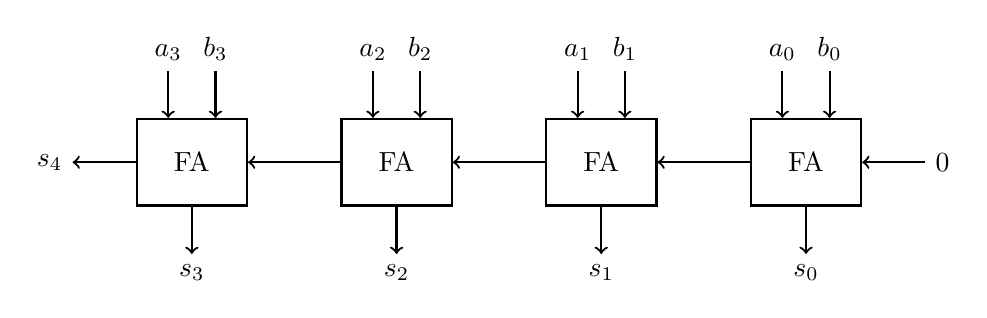
\begin{tikzpicture}[fa/.style={draw, thick, minimum width=1.4cm, minimum height=1.1cm}]
  \foreach \i in {0,1,2,3}{
    \node[fa] (f\i) at ({-2.6*\i},0) {FA};
    \draw[<-, thick] ([xshift=-0.3cm]f\i.north) -- ++(0,0.6) node[above]{$a_\i$};
    \draw[<-, thick] ([xshift=0.3cm]f\i.north) -- ++(0,0.6) node[above]{$b_\i$};
    \draw[->, thick] (f\i.south) -- ++(0,-0.6) node[below]{$s_\i$};
  }
  \foreach \i/\j in {0/1,1/2,2/3}{
    \draw[->, thick] (f\i.west) -- (f\j.east);
  }
  \draw[<-, thick] (f0.east) -- ++(0.8,0) node[right]{0};
  \draw[->, thick] (f3.west) -- ++(-0.8,0) node[left]{$s_4$};
\end{tikzpicture}
\caption{A 4-bit ripple-carry adder. Bit 0 is the least significant bit, on the right. The final
carry out becomes the fifth bit of the answer.}
\label{fig:ripple}
\end{figure}

The carry ``ripples'' from right to left, just as it does when you add with a pencil. A 64-bit adder
is simply 64 full adders in a row.

\section{Checking the Design in Python}
Before a company spends millions of dollars making a chip, engineers simulate every circuit. Let us do the
same. The program below defines a single gate, \pyfunction{nand}, and builds everything else from it.
It even counts how many NAND gates it uses. Create a file called \filename{adder.py}:

\begin{minted}{python}
nand_count = 0

def nand(a, b):
    global nand_count
    nand_count += 1
    return 0 if (a == 1 and b == 1) else 1

# Every other gate is built from NAND
def not_(a):
    return nand(a, a)

def and_(a, b):
    return not_(nand(a, b))

def or_(a, b):
    return nand(not_(a), not_(b))

def xor(a, b):
    n = nand(a, b)
    return nand(nand(a, n), nand(b, n))

def full_adder(a, b, carry_in):
    s = xor(a, b)
    total = xor(s, carry_in)
    carry_out = or_(and_(a, b), and_(s, carry_in))
    return total, carry_out

def add(a_bits, b_bits):
    # Bits are listed from least significant to most significant
    carry = 0
    result = []
    for a, b in zip(a_bits, b_bits):
        total, carry = full_adder(a, b, carry)
        result.append(total)
    result.append(carry)
    return result

def to_bits(n, width):
    return [(n >> i) & 1 for i in range(width)]

def to_int(bits):
    return sum(bit << i for i, bit in enumerate(bits))

print("6 + 7 =", to_int(add(to_bits(6, 4), to_bits(7, 4))))

# Test every pair of 4-bit numbers
errors = 0
for x in range(16):
    for y in range(16):
        if to_int(add(to_bits(x, 4), to_bits(y, 4))) != x + y:
            errors += 1
print("pairs tested: 256, errors:", errors)

nand_count = 0
add(to_bits(6, 4), to_bits(7, 4))
print("NAND gates used for one 4-bit addition:", nand_count)
\end{minted}

The names \pyfunction{not\_}, \pyfunction{and\_}, and \pyfunction{or\_} end with an underscore because
\texttt{not}, \texttt{and}, and \texttt{or} are already Python keywords. The function \pyfunction{to\_bits}
uses \texttt{>>} (shift right) and \texttt{\&} (bitwise AND) to pull out one bit at a time.

When you run it, you should see:
\begin{verbatim}
6 + 7 = 13
pairs tested: 256, errors: 0
NAND gates used for one 4-bit addition: 60
\end{verbatim}

Every one of the 256 possible additions is correct. Our straightforward full adder uses
$4 + 4 + 2 + 2 + 3 = 15$ NAND gates, so 4 bits take 60. The clever 9-gate version is an exercise.

\section{Subtraction for Free}\index{subtraction!in hardware}
In the Data Representation chapter, you learned that in two's complement, you negate a number by
flipping every bit and adding 1. So
$$A - B = A + (\text{flipped } B) + 1$$
A chip does not need a separate subtracting circuit. It runs $B$ through a row of inverters and sets the
carry into the rightmost full adder to 1 instead of 0. That ``$+1$'' comes for free.

\section{From Adders to Computers}
Your adder is the core of the \newterm{arithmetic logic unit} (ALU),\index{arithmetic logic unit} the part
of a processor that does the math. A few more ideas turn it into a computer:
\begin{itemize}
\item \textbf{Memory.} Wire two NAND gates in a loop, each feeding the other, and the pair can hold a
bit after its inputs go away. Thousands of these store the numbers being added.
\item \textbf{A clock.} A signal that ticks billions of times per second tells every part when to
take its next step.
\item \textbf{Control.} Instructions, stored as bits like everything else, choose which operation the
ALU performs on each tick.
\end{itemize}

A modern phone chip holds tens of billions of transistors. Each one is just a switch, but arranged
the right way, they add, compare, store, and decide. That is how a computer actually computes.

\begin{Exercise}[title={NOR Truth Table}, label=dl_nor]
Make a truth table for $\neg(A \text{ or } B)$. Which gate is this?
\end{Exercise}
\begin{Answer}[ref=dl_nor]
\begin{tabular}{c c | c}
$A$ & $B$ & out \\
\hline
0 & 0 & 1 \\
0 & 1 & 0 \\
1 & 0 & 0 \\
1 & 1 & 0 \\
\end{tabular}

It is the NOR gate: the output is 1 only when both inputs are 0.
\end{Answer}

\begin{Exercise}[title={NOR Is Universal Too}, label=dl_noruniv]
Show how to build NOT and OR using only NOR gates.
\end{Exercise}
\begin{Answer}[ref=dl_noruniv]
NOT: NOR$(A, A) = \neg(A \text{ or } A) = \neg A$.

OR: a NOR followed by a NOR used as a NOT: NOR$\big(\text{NOR}(A,B), \text{NOR}(A,B)\big) = A \text{ or } B$.
That is 2 NOR gates. (AND then follows from De Morgan's law: $A \text{ and } B = \text{NOR}(\neg A, \neg B)$.)
\end{Answer}

\begin{Exercise}[title={Add by Hand}, label=dl_add]
Add $1011_2$ and $0110_2$ in binary. Check your answer in decimal. Why does the answer need 5 bits?
\end{Exercise}
\begin{Answer}[ref=dl_add]
$1011_2 + 0110_2 = 10001_2$. In decimal, $11 + 6 = 17 = 16 + 1$. The largest 4-bit number is 15, so 17
does not fit; the final carry out becomes the fifth bit.
\end{Answer}

\begin{Exercise}[title={Trace a Full Adder}, label=dl_trace]
Find the sum and carry out of a full adder when $A = 1$, $B = 1$, and $C_{\text{in}} = 1$, using the two
formulas for a full adder.
\end{Exercise}
\begin{Answer}[ref=dl_trace]
$A \oplus B = 0$, so sum $= 0 \oplus 1 = 1$. $C_{\text{out}} = (1 \text{ and } 1) \text{ or } (0 \text{ and } 1)
= 1$. The carry and sum are 1 and 1: in binary, $1 + 1 + 1 = 11_2 = 3$.
\end{Answer}

\begin{Exercise}[title={Counting Transistors}, label=dl_count]
Using 9 NAND gates per full adder and 4 transistors per NAND gate, how many transistors does a 64-bit
ripple-carry adder need?
\end{Exercise}
\begin{Answer}[ref=dl_count]
$64 \times 9 = 576$ NAND gates, and $576 \times 4 = 2{,}304$ transistors. That is a tiny fraction of a modern
chip.
\end{Answer}

\begin{Exercise}[title={The Clever Full Adder}, label=dl_nine]
Rewrite \pyfunction{full\_adder} to use only 9 NAND gates. Check that the test still finds 0 errors
and that the count drops to 36.

Hint: build each XOR from 4 NANDs, and save the output of the first gate of each:
$$n_1 = \text{NAND}(A, B)$$
$$m_1 = \text{NAND}(A \oplus B, C_{\text{in}})$$
Then $C_{\text{out}} = \text{NAND}(n_1, m_1)$.
\end{Exercise}
\begin{Answer}[ref=dl_nine]
\begin{minted}{python}
def full_adder(a, b, carry_in):
    n1 = nand(a, b)
    s = nand(nand(a, n1), nand(b, n1))
    m1 = nand(s, carry_in)
    total = nand(nand(s, m1), nand(carry_in, m1))
    carry_out = nand(n1, m1)
    return total, carry_out
\end{minted}
The test still reports 0 errors, and a 4-bit addition now uses $4 \times 9 = 36$ NAND gates. The trick
works because, by De Morgan's law, NAND$(n_1, m_1)$ is $(A \text{ and } B)$ or $((A \oplus B) \text{ and }
C_{\text{in}})$.
\end{Answer}

\begin{Exercise}[title={Waiting for the Carry}, label=dl_ripple]
Each gate takes a tiny amount of time to switch. Why is a ripple-carry adder slow for 64-bit numbers?
\end{Exercise}
\begin{Answer}[ref=dl_ripple]
The leftmost full adder cannot finish until its carry in is known, which waits on the adder to its right,
and so on down the line. In the worst case (for example, adding 1 to a number that is all 1s), the carry
must pass through all 64 full adders, one after another. Real chips use \emph{carry-lookahead} adders, which
spend extra gates to figure out the carries in parallel.
\end{Answer}

\begin{Exercise}[title={Subtract with an Adder}, label=dl_sub]
Write a function \pyfunction{subtract} that takes two lists of bits, flips every bit of the second
list with \pyfunction{not\_}, starts the carry at 1, and adds. Use it to compute $13 - 6$ with
4 bits.
\end{Exercise}
\begin{Answer}[ref=dl_sub]
\begin{minted}{python}
def subtract(a_bits, b_bits):
    carry = 1
    result = []
    for a, b in zip(a_bits, b_bits):
        total, carry = full_adder(a, not_(b), carry)
        result.append(total)
    return result

print(to_int(subtract(to_bits(13, 4), to_bits(6, 4))))   # 7
\end{minted}
It prints 7. The final carry is dropped, because a 4-bit two's complement answer has only 4 bits.
\end{Answer}
